%!TEX root = ../USthesis_Masters.tex
\chapter{System Design}
\label{chp:System Design}


%%%%%%%%%%%%%%%%%%%%%%%%%%%%%%%%%%%%%%%%%%%%%%%%%%%%%%%%%%%%%%%%%%%%%%%
\section{Framework}

In this project we test the viability of a payment framework on a mobile social media platform. The framework will consist of several connected pieces.

A REST API will form the core of the framework. It will be responsible for managing payment request made by clients that use the framework.

The REST API will be accompanied by a wallet application that will be directly connected to the REST API. This will allow a user to reference a payment request from the wallet application to simplify the payment process for the user.

To practically test the payment framework, we will create a use-case application that will use the framework to sell virtual gamebooks. 

% \begin{itemize}
% 	\item REST API for payments
% 	\item Wallet Application
% 	\item Bitcoin Interface
% 	\item Use-case Application
% \end{itemize}

A summary of what is required from the system can be seen in figure \ref{fig:summary_framework}.

\begin{figure}
  \centering
  	\caption{Interaction between the parts of the system.} 
    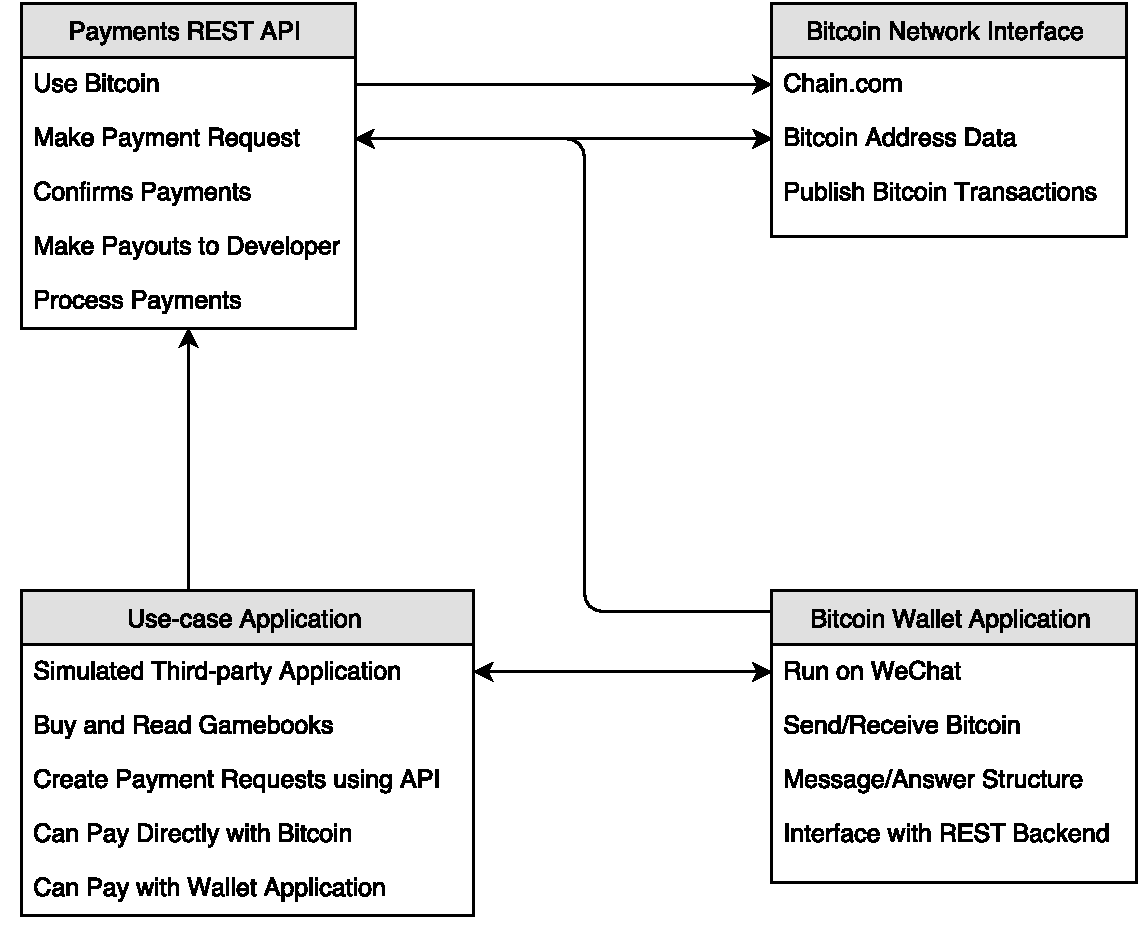
\includegraphics[width=0.7\textwidth]{figs/Summary.pdf}
   
   \label{fig:summary_framework}
\end{figure}

\subsection{REST API for payment management}

A REST (Representational State Transfer) API \cite{Oracle.com} was chosen for the main interface for developers to use Bitcoin without running a Bitcoin node or having experience with Bitcoin. REST was chosen because it is a commonly used architecture, it is easy to use and understand and it does not constrain the user's choice of programming language or environment. 

An alternative to REST is SOAP (Simple Object Access Protocol) \cite{Box2000}. REST was chosen above SOAP due to the fact that REST uses existing generic web interfaces \cite{Fielding2000}. REST was also chosen due to the author's familiarity with the architecture.

The purpose of the REST API is to let developers make payment requests and check if a payment has been made, without dealing with the low-level Bitcoin transactions directly. Therefore, the system should generate a new Bitcoin address on request. 

The payment requests that are made by developers are the resources of the REST API. A payment request will consist of a Bitcoin address to receive payment and a payment identifier number to reference the payment. It will also contain information about the payment, like the amount to be paid, a lable that describes the payment and the status of the payment.

For simplicity sake, we will only use the HTTP methods POST and GET to create and retrieve resources, respectively. We will not implement the PUT and DELETE methods, since changing or deleting a payment resource is not necessary for the payment framework to function.
% We also require the developer to check wether a payment has been successfully made.
% THe requirements for the REST API are:

% \begin{itemize}
% 	\item New Bitcoin address for each payment
% 	\item Verify payment
% 	\item Check total balance of developer
% 	\item Withdraw available Bitcoin of developer
% \end{itemize}

% \subsubsection{The concept of the Bitcoin payment}

% This is a high-level explanation of how to receive verifyable payments with Bitcoin. With Bitcoin, unlike a traditional bank account, the user does not have a single ``account'' where people can make payments to and one can verify that the payment came from them. With Bitcoin it is trivially easy to make a new Bitcoin address, and it can be generated without being connected to the Internet or the Bitcoin network.

% Since the entire Bitcoin blockchain is public, a single address is not sufficient to receive multiple payments. With a single address, it is not easy to verify that a specific person has made a payment, since there may be several payments of the same amount happening in short succession.

% The solution to the problem is generating a new address for every payment, and requesting that the user make the payment to that address. Since the newly generated address is not yet present on the blockchain, when a payment to that address of the requested amount occurs, it can be certain that the person in question made the payment. When the payment is complete, the Bitcoin in that address can be transferred to a central address, and the original address can be discarded.

% From the requirements for the REST API, we clearly require (at least) the following methods:

% \begin{itemize}
% 	\item A payment method
% 	\item A balance method
% 	\item A payout method
% \end{itemize}

As mentioned in chapter \ref{rest}, REST uses URIs to reference resources. A specific part of the URI that identifies the resource will be referred to as an ``endpoint'' in the rest of this chapter. The URI contains the domain name and other information that is used in every request that do not identify the specific request.

\subsubsection{The /payment endpoint}
\label{sct:payment}

The /payment endpoint is the core of the REST API. It is used to make a payment request with a specified amount of Bitcoin and a description of the transaction. The /payment endpoint returns a Bitcoin public address and a payment ID. 

The user can then pay to the Bitcoin address using any standard Bitcoin payment endpoint, or can pay directly from the Bitcoin wallet that will run on WeChat and will be connected to the payment infrastructure.

\subsubsection{/payment/\{PUBLIC\_ADDRESS\} and /payment/\{ID\}}

These two methods are conceptually the same, but they take in two different arguments. The first one takes the Bitcoin address to be queried, and the second one takes the payment ID. They both return all the data about the transaction, including the status of the transaction. 

The main purpose of this endpoint is to verify that a transaction has been completed by the user. It can also be used to give the payment details to user again.

\subsubsection{/balance}

The /balance endpoint gives the developer the balance of all the available Bitcoin from all the received transactions. The endpoint also returns a flag that says if there is enough Bitcoin to make a payout.

\subsubsection{/payout}

The /payout endpoint is used by the developer to transfer all of the available Bitcoin to a specified Bitcoin address.

\subsection{Wallet Application}

The Wallet Application is a Bitcoin wallet implemented on the WeChat platform. The WeChat platform uses a simple message-answer structure. A user sends a message in the Wallet Application. The message is then sent to WeChat that sends it to a third party server controlled by the developer. The server then sends a reply to WeChat that is then forwarded to the user. 

In this manner, a fully functional Bitcoin wallet is realised. The third party server stores the private keys and processes the Bitcoin transactions on commands from the user.

The advantage of using the WeChat platform is the security built into the platform, as well as an existing user base. 

The Wallet Application will be directly connected to the back-end of the REST API. Every payment request is asociated with an unique ID. Therefore, payment requests will be accessible directly from the Wallet Application by using the ID in conjunction to referencing a Bitcoin address. 

\subsection{Bitcoin Interface}
\label{sct:bitcoin_interface}

To connect to the Bitcoin peer-to-peer network, a Bitcoin client is needed. The standard way of doing this is running the Bitcoin open source software on a server. This is very network and processor intensive. For development and testing for this project, it will be quite expensive to run the Bitcoin software. According to a test done in July 2014 \cite{Halliday}, running a full Bitcoin node Amazon Web Services cost \$42.06 in a month. The node used about 135GB of data transfer that cost \$19.46. The data transfer is also dependant on the amount of Bitcoin transactions that are made, so the price may vary.

The price of running a Bitcoin node is acceptable when running a production service that requires it, but for the purposes of testing the viability of Bitcoin on a social media platform, we do not need a full Bitcoin node.

 Therefore, an alternative is required for interfacing with the Bitcoin network. Fortunately, there are services that provide access to most of the Bitcoin operations using their APIs. 

Such a service must be able to get the balance and unspent outputs of a Bitcoin address. It should also be able to post a Bitcoin transaction to the Bitcoin network. For our testing purposes, this service must also be able to use the Bitcoin testnet. The Bitcoin testnet is an alternative blockchain that functions almost identically to the standard blockchain, but is designed not to have any value to allow developers to build Bitcoin systems without using real Bitcoin \cite{testnet}. 

% The following is required from such a service:

% \begin{itemize}
% 	\item Get the balance from an address,
% 	\item Get unspent outputs from an address,
% 	\item Post a signed Bitcoin transaction to the network,
% 	\item It must be able to use the Testnet
% \end{itemize}

The details of the chosen service is covered in chapter \ref{chp:Detail Design}.
% After considering several options, a service called chain.com was chosen. Chain.com is a free service that satisfies all the requirements. It is perfect to use this service as a proof of concept, but in practice one would rather run a full Bitcoin node to minimize reliance on third-party services.

\subsection{Use-case Application}

To use the payment framework, a Gamebook application is created to read Choose Your Own Adventure style books \cite{cyoa} on the WeChat platform. User-created books can be sold by using the Bitcoin payment framework and the author can potentially earn Bitcoin.

For each sale, the Gamebook application creates a payment request using the REST API. The user can then pay using the Wallet Application or any Bitcoin payment mechanism. The Gamebook application can then query the API to confirm that the payment is received. 

When the payment has been received, the user will then be able to read a gamebook that they bought using Bitcoin on their phone. The interaction between the Gamebooks application and the rest of the system can be seen in figure \ref{fig:summary_framework}.

Accompanying the Gamebook application, we will design a Gamebook author webpage to allow people to write the gamebooks that will be available on the application. With this design, it would be possible for authors to write and publish gamebooks and be paid for their work by the readers that buy the gamebook.